\documentclass{beamer}
\usepackage[utf8]{inputenc}

\usetheme{Madrid}
\usecolortheme{default}
\usepackage{amsmath,amssymb,amsfonts,amsthm}
\usepackage{txfonts}
\usepackage{tkz-euclide}
\usepackage{listings}
\usepackage{adjustbox}
\usepackage{array}
\usepackage{tabularx}
\usepackage{gvv}
\usepackage{lmodern}
\usepackage{circuitikz}
\usepackage{tikz}
\usepackage{graphicx}
\usepackage{enumitem}

\setbeamertemplate{page number in head/foot}[totalframenumber]

\usepackage{tcolorbox}
\tcbuselibrary{minted,breakable,xparse,skins}



\definecolor{bg}{gray}{0.95}
\DeclareTCBListing{mintedbox}{O{}m!O{}}{%
  breakable=true,
  listing engine=minted,
  listing only,
  minted language=#2,
  minted style=default,
  minted options={%
    linenos,
    gobble=0,
    breaklines=true,
    breakafter=,,
    fontsize=\small,
    numbersep=8pt,
    #1},
  boxsep=0pt,
  left skip=0pt,
  right skip=0pt,
  left=25pt,
  right=0pt,
  top=3pt,
  bottom=3pt,
  arc=5pt,
  leftrule=0pt,
  rightrule=0pt,
  bottomrule=2pt,
  toprule=2pt,
  colback=bg,
  colframe=orange!70,
  enhanced,
  overlay={%
    \begin{tcbclipinterior}
    \fill[orange!20!white] (frame.south west) rectangle ([xshift=20pt]frame.north west);
    \end{tcbclipinterior}},
  #3,
}
\lstset{
    language=C,
    basicstyle=\ttfamily\small,
    keywordstyle=\color{blue},
    stringstyle=\color{orange},
    commentstyle=\color{green!60!black},
    numbers=left,
    numberstyle=\tiny\color{gray},
    breaklines=true,
    showstringspaces=false,
}
%------------------------------------------------------------
%This block of code defines the information to appear in the
%Title page
\title %optional
{2.5.5}
\date{September 6, 2025}

\author 
{Shreyas Goud Burra - EE25BTECH11051}

\begin{document}

\frame{\titlepage}
\begin{frame}{Question}
    Write the projection of the vector ($\vec{b} + \vec{c}$) on the vector $\vec{a}$, where $\vec{a} = 2\hat{i}-2\hat{j}+\hat{k}$, $\vec{b} = \hat{i}+2\hat{j}-2\hat{k}$, and $\vec{c} = 2\hat{i}-\hat{j}+4\hat{k}$.\\
\end{frame}

\begin{frame}{Given Information}
    Let the vectors be represented as \textbf{A}, \textbf{B}, and \textbf{C} respectively. Given by

\begin{align}
    \textbf{A} = \myvec{2 \\ -2 \\ 1}, \textbf{B} = \myvec{1 \\ 2\\ -2}, \textbf{C} = \myvec{2\\-1\\4}
    \label{0.1}
\end{align}
\end{frame}

\begin{frame}{Solution}
    Mathematically, the projection of the vector \textbf{B}+\textbf{C} on the vector \textbf{A} is given by some vector \textbf{D},

\begin{align}
    \textbf{D} = k\textbf{A}\text{, such that } ((\textbf{B}+\textbf{C})-\textbf{D})^\text{T}\textbf{D}=0
    \label{0.2}
\end{align}
\end{frame}

\begin{frame}{Continuation}
    yielding,

\begin{align}
    ((\textbf{B}+\textbf{C})-k\textbf{A})^\text{T}\textbf{A}=0
    \label{0.3}
\end{align}

or,


\begin{align}
    k=\frac{(\textbf{B}+\textbf{C})^\text{T}\textbf{A}}{\norm{\textbf{A}}^2} \implies \textbf{D} = \frac{(\textbf{B}+\textbf{C})^\text{T}\textbf{A}}{\norm{\textbf{A}}^2}\textbf{A}
    \label{0.4}
\end{align}
\end{frame}

\begin{frame}{Continuation}
    On substituting the values,

\begin{align}
    \textbf{D} = \frac{\brak{\myvec{1\\2\\-2}+\myvec{2\\-1\\4}}^\text{T}\myvec{2\\-2\\1}}{\norm{\myvec{2\\-2\\1}}^2}\myvec{2\\-2\\1}
    \label{0.5}
\end{align}
\end{frame}

\begin{frame}{Final Answer}
    On calculation, this gives us,

\begin{align}
    \textbf{D} = \myvec{4/3\\-4/3\\2/3}
    \label{0.6}
\end{align}
\end{frame}

\begin{frame}[fragile]
\frametitle{C code}
\begin{lstlisting}

#include <stddef.h>
#include<math.h>

void project(double* result, const double* arr2, const double* arr3, int length) {
    float dot_product = 0.0f;
    float magnitude_squared = 0.0f;
    
    for (int i = 0; i < length; i++) {
        dot_product += arr2[i] * arr3[i];
    }

    
    for (int i = 0; i < length; i++) {
        magnitude_squared += arr3[i] * arr3[i];
    }

\end{lstlisting}
\end{frame}

\begin{frame}[fragile]
\frametitle{C code}
\begin{lstlisting}

    
    if (magnitude_squared == 0.0f) {
        for (int i = 0; i < length; i++) {
            result[i] = 0.0f;
        }
        return;
    }

    
    const float scalar = dot_product / magnitude_squared;

\end{lstlisting}
\end{frame}

\begin{frame}[fragile]
\frametitle{C code}
\begin{lstlisting}

    
    for (int i = 0; i < length; i++) {
        result[i] = scalar * arr3[i];
    }

    for(int i=0; i<length; i++){
	result[i] = floor(result[i] * 100) / 100;
    }
}

\end{lstlisting}
\end{frame}

\begin{frame}[fragile]
\frametitle{Python code}
\begin{lstlisting}

import numpy as np
import matplotlib.pyplot as plt
import ctypes
import os
import sys

project_lib = ctypes.CDLL('./project.so')
project_lib.project.argtypes = [
        ctypes.POINTER(ctypes.c_double),
        ctypes.POINTER(ctypes.c_double),
        ctypes.POINTER(ctypes.c_double),
        ctypes.c_int
]

project_lib.project.restype = ctypes.c_double

\end{lstlisting}
\end{frame}

\begin{frame}[fragile]
\frametitle{C code}
\begin{lstlisting}

#E = B+C

A=np.array([2, -2, 1], dtype=np.float64)
B=np.array([1, 2, -2], dtype=np.float64)
C=np.array([2, -1, 4], dtype=np.float64)
D=np.zeros(3, dtype=np.float64)
E=B+C

m=len(A)

\end{lstlisting}
\end{frame}

\begin{frame}[fragile]
\frametitle{Python code}
\begin{lstlisting}

project=project_lib.project(
        D.ctypes.data_as(ctypes.POINTER(ctypes.c_double)),
        E.ctypes.data_as(ctypes.POINTER(ctypes.c_double)),
        A.ctypes.data_as(ctypes.POINTER(ctypes.c_double)),
        m
)


fig=plt.figure()
ax=fig.add_subplot(111, projection='3d')

ax.quiver(0, 0, 0, E[0], E[1], E[2], color='b', arrow_length_ratio=0.1)
ax.quiver(0, 0, 0, A[0], A[1], A[2], color='r', arrow_length_ratio=0.1)
ax.quiver(0, 0, 0, D[0], D[1], D[2], color='g', arrow_length_ratio=0.2)

\end{lstlisting}
\end{frame}

\begin{frame}[fragile]
\frametitle{Python code}
\begin{lstlisting}


label = f'({A[0]}, {A[1]}, {A[2]})'
ax.text(A[0], A[1], A[2], s=label, color='b', fontsize=10)

label = f'({E[0]}, {E[1]}, {E[2]})'
ax.text(E[0], E[1], E[2], s=label, color='b', fontsize=10)

label = f'({D[0]}, {D[1]}, {D[2]})'
ax.text(D[0], D[1], D[2], s=label, color='b', fontsize=10)

\end{lstlisting}
\end{frame}
\begin{frame}[fragile]
\frametitle{C code}
\begin{lstlisting}

ax.scatter(A[0], A[1], A[2], color='r', s=50)
ax.scatter(E[0], E[1], E[2], color='b', s=50)
ax.scatter(D[0], D[1], D[2], color='g', s=50)

ax.set_xlim([0, 4])
ax.set_ylim([-4, 4])
ax.set_zlim([-4, 4])

\end{lstlisting}
\end{frame}

\begin{frame}[fragile]
\frametitle{Python code}
\begin{lstlisting}

ax.set_xlabel('X-axis')
ax.set_ylabel('Y-axis')
ax.set_zlabel('Z-axis')

plt.title('Vector Projection')

plt.savefig('/home/shreyas/GVV_Assignments/matgeo/2.5.5/figs/fig1.png')

plt.show()
\end{lstlisting}
\end{frame}

\begin{frame}{Plot}
    \begin{figure}[H]
    \centering
    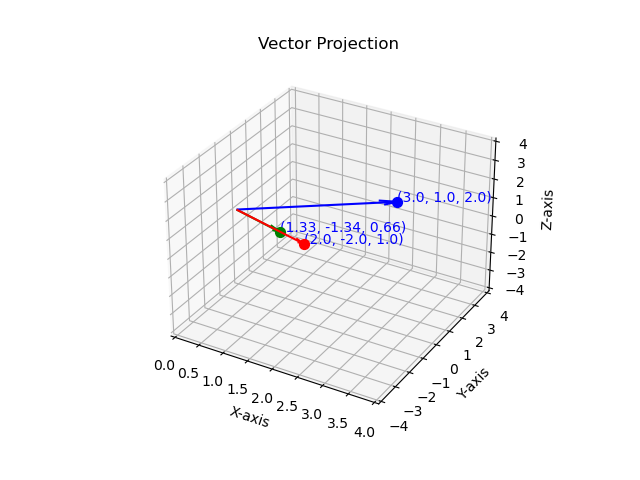
\includegraphics[width=0.8\columnwidth]{figs/fig1.png}
    \caption{3D Plot}
    \label{3D Plot}
\end{figure}
\end{frame}
\end{document}
